\documentclass[fontsize=9pt]{slnotes}
\usepackage{wrapfig}

\newfontfamily{\symbolfont}{DejaVu Sans}[Scale=MatchLowercase]
\DeclareTextFontCommand{\textsymbol}{\symbolfont}

\newcommand\benefits{\checkmark}
\newcommand\problems{\textsymbol{✗}}

\newcommand\sltilde{\char`~}
\begin{document}
\chapter{CS2106: Basic ideas}
The first computers did not have OSes. Rudimentary OSes like batch OSes that executed programs one at a time developed in the 1960s. Time-sharing OSes came in the 1970s.

OSes abstract away hardware, manage resources, control program execution and provide security and protection.

\sldef{Monolithic kernels} are kernels where the entire kernel runs in kernel mode. This design is well understood and tends to have better performance, but components tend to be more coupled and usually have complicated internal structures. Most Unices are largely monolithic.

\sldef{Microkernels} are kernels where the kernel is very small and handles only basic services like IPC, interrupt handling, and memory and task management. Higher level services run in user space, built on top of the basic facilities. This usually leads to a more robust kernel with better isolation, but performance tends to be lower.

\sldef{Layered systems} are generalisations of monolithic kernels that could be seen as a cross between microkernels and monolithic kernels: most services still run in kernel mode, but they are divided into layers, with the lowest being the hardware abstraction layer, and higher layers making use of lower layers. NT is generally seen as a layered system.

The \sldef{client-server model} is a variation of a microkernel. Servers are built on top of the microkernel and client processes request services from servers. Client and server processes can be on separate machines.

\sldef{Virtualisation} is used to run multiple OSes on the same hardware, or to debug an OS. Using a \sldef{hypervisor}, underlying hardware is virtualised. A \sldef{type 1} \sltilde{} is one that runs directly on hardware; a \sldef{type 2} \sltilde{} runs on a host OS.

\chapter{Processes}
A \sldef{process}/task/job is an abstraction to represent a program in execution.

Each \sltilde{} is represented in the system process table by a \sldef{process control block} which contains the register state (PC, SP, FP, GPRs, etc.), memory region information, PID, process state, etc.

CS2106 models processes as having 5 states: new, ready, running, blocked, and terminated.

\begin{wrapfigure}{l}{0.5\columnwidth}
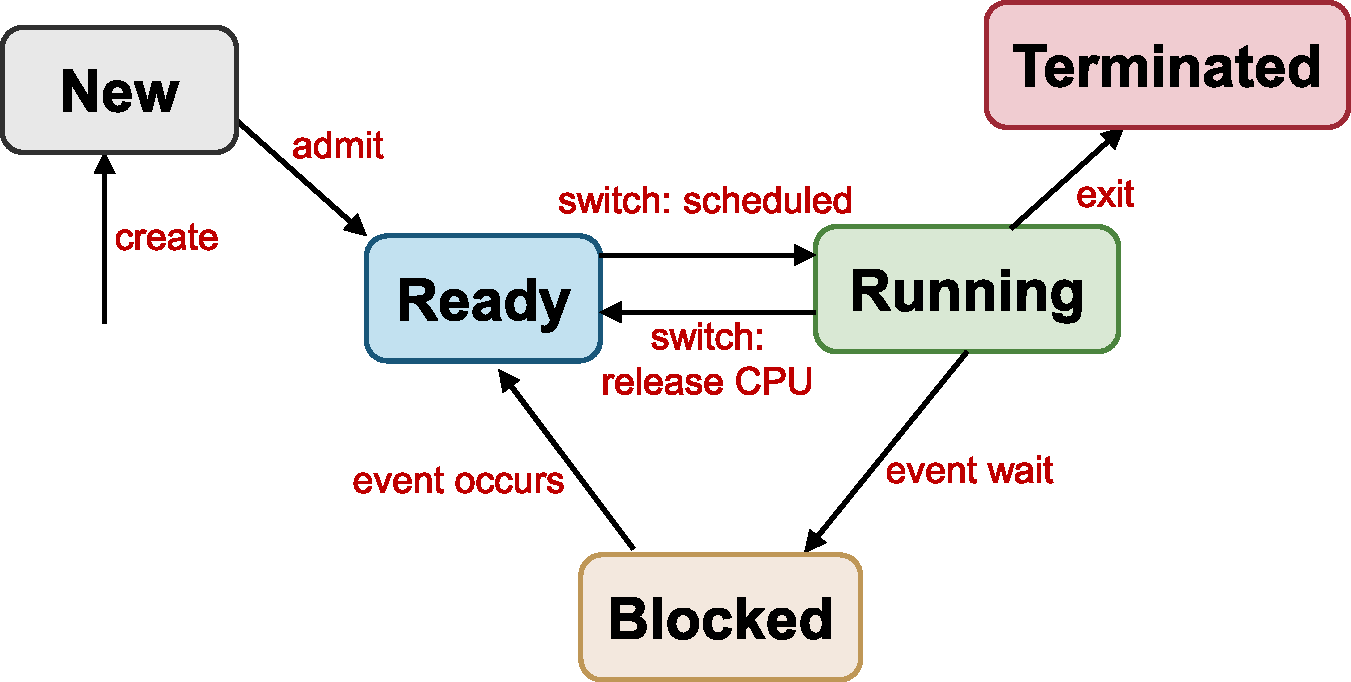
\includegraphics[width=0.5\columnwidth]{pstates.pdf}
\end{wrapfigure}

A \sldef{syscall} is a request by a program for the system to do something. A change from user to kernel mode needs to happen. The general mechanism is \begin{slinenum}
\item program calls library
\item library performs syscall convention e.g. syscall no. in register, then execute special instruction
\item syscall entry dispatches to correct handler
\item syscall is executed
\item returns to user mode
\item library returns
\end{slinenum}.

An \sldef{exception} is a synchronous event caused by program execution e.g. arithmetic errors or segmentation faults; an exception handler (in the kernel) is executed. An \sldef{interrupt} is an external event e.g. timers or mouse/keyboard events; they are asynchronous and occur independently of program execution; program execution is suspended and an interrupt handler is executed.

Each task has a \sldef{stack} that keeps track of e.g. return address, function arguments, local variables, saved registers (register spilling when GPRs are exhausted).

A \sldef{calling convention} determines what the caller and callee does to set up the stack frame, how to pass arguments, what registers are saved by who, etc.

\section{Unix process abstraction}
\texttt{int fork()} creates a child process by duplicating the current process. Linux has \texttt{clone()} that allows more fine-grained control.

The \texttt{exec} family replaces the currently running program with a new one.

\texttt{void \_exit(int status)} ends the current process with the given status.

\texttt{pid\_t wait(int *wstatus)} waits for a child process to terminate; \texttt{pid\_t waitpid(pid\_t pid, int *wstatus, int options)} waits for (possibly) a specific child process; \texttt{waitid} waits for any child to change status.

When a process exits, it becomes a zombie process until its parent \texttt{wait()}s on it. If a process exits before child processes exit, the children will be inherited by \texttt{init}.

Linux process states: ready, running, stopped, suspended/sleeping, zombie.

\chapter{Scheduling}
\sldef{Concurrency} could be virtual i.e. pseudoparallelism, or physical: multi- or multicore CPUs. CS2106 does not really distinguish.

\sldef{Scheduling problem}: if there are more ready processes than CPUs, which should run?

3 categories of processing environments: batch i.e. no user so no need to be responsive, interactive/multiprogramming i.e. with user interaction so should be responsive, and realtime i.e. have hard deadline.

All \sltilde{} should have \begin{slinenum}
\item fairness i.e. each process/user gets a fair share of CPU and no starvation
\item balance i.e. all parts of the system should be used
\end{slinenum}

Two types of multitasking: \begin{slinenum}
\item \sldef{cooperative/non-preemptive}: processes run until blocked or voluntarily yield
\item \sldef{preemptive}: processes have fixed time quota (still can block or yield) and are scheduled out when quota is used
\end{slinenum}.

Process scheduling: \begin{slinenumthen}
\item scheduler triggered
\item context switch occurs if needed
\item scheduling algorithm picks process to run
\item process's context is set up
\item process runs
\end{slinenumthen}

\section{Batch processing scheduling}
Criteria: \begin{slinenum}
\item turnaround time: total time from submission to completion
\item throughput: rate of task completion
\item CPU utilitisation: \% of time CPU is working on a task
\end{slinenum}.

\sldef{FCFS}: arriving tasks are enqueued in a simple FIFO queue, and the head of the queue is run until done/block/yield. Guaranteed to have no starvation. \problems: convoy effect: if task A is CPU-bound and followed by a number of IO-bound tasks X, then while A is running Xs are waiting (IO idle) and when A is blocked on IO, Xs all run and then get blocked waiting for IO (CPU idle).

\sldef{Shortest job first}: select task with smallest total CPU time. Need to know total CPU time in advance, or guess. This minimises average waiting time, but starvation is possible; a long job may never be scheduled.

A common approach to predicting is an exponential average: \(P_{n+1} = \alpha A_n + (1-\alpha) P_n\), where \(\alpha\) is the weight placed on recent events.

\sldef{Shortest remaining time}: variant of SJF, using the shortest remaining time instead. It is preemptive: a new job with a shorter remaining time can preempt a currently running task.

\section{Interactive scheduling}
Criteria: \begin{slinenum}
\item response time: time between request and response
\item predictability: minimise variation in response time
\end{slinenum}.

To ensure good response time, preemptive scheduling algorithms are used. In order to preempt, the scheduler needs to run periodically, using a timer interrupt and a handler that invokes the scheduler.

The \sldef{interval of timer interrupt} (ITI) is the interval between timer interrupts. The \sldef{time quantum} is the execution duration given to a process, which must be multiples of the ITI, and could be constant or variable among processes.

\sldef{Round-robin}: tasks stored in FIFO queue, and run until TQ/yield/block. Response time bounded by \((n-1)q\) where \(q\) is TQ. Choice of TQ is important: high has lower overhead but longer waiting time, and v.v.

\sldef{Priority}: Select task with highest priority. Can be preemptive i.e. late high-prio task can preempt low-prio running task, or non-preemptive i.e. has to wait for next scheduling. \problems: low-prio task can starve; solutions: decrease prio of running task after each TQ, or don't consider current running task in next scheduling if TQ expires.

\sldef{Priority inversion}: If lower prio task preempts higher prio task e.g. high A, B, low C, C starts and locks file, B preempts C, A arrives and needs file but locked by C, so B runs even though A has higher prio.

\sldef{Multi-level feedback queue}: Adapts to process behaviour and minimises response (for IO-bound) and turnaround (for CPU-bound) time. Rules: if \(p(A) > p(B)\) then A runs; if \(p(A) == p(B)\) then A and B run in RR. New tasks start at highest prio; tasks that finish TQ drop prio, but if yield/block before TQ then keep prio. \problems: too many interactive tasks can cause long-running tasks to starve; can be gamed if tasks yield just before TQ; task that stops being CPU-bound stays at low prio. Solutions: periodic priority boost, and account overall time usage, and drop prio when that exceeds allotment.

\sldef{Lottery}: Give tickets to processes for resources, and choose tickets randomly when scheduling. It \begin{slinenum}
\item is responsive: new tasks can participate in the next lottery
\item provides good control: can vary tickets per task
\item is simple in implementation
\end{slinenum}.

\chapter{IPC}
\sldef{Shared memory}: communicate using a memory region mapped to multiple tasks. Advantages: efficient (OS only involved in initial steps) and easy to use. Disadvantages: synchronisation is hard because it is a shared resource.

POSIX shared memory: \begin{slinenum}
\item \texttt{int shmget(key, size, shmflg)} returns the ID of a new or existing shared memory segment (to create, \texttt{key = IPC\_PRIVATE}, \texttt{shmflg = IPC\_CREAT | <octal permissions>})
\item \texttt{void *shmat(shmid, shmaddr, shmflg)} attaches the specified SHM to \texttt{shmaddr} or a suitable address if null
\item \texttt{int shmdt(shmaddr)} detaches the SHM at the address
\item \texttt{int shmctl(shmid, cmd, ...)} destroys the SHM if \texttt{cmd} is \texttt{IPC\_RMID} (only for owner/creator)
\end{slinenum}.

\sldef{Message passing}: passing message via (usually) syscalls. Messages have to be stored in kernel memory, and each operation is a syscall. Naming: either direct or indirect i.e. via mailboxes or ports, which can be shared. Sync/async: sync means sender/receiver is blocked until message is received/sent; async means sender resumes immediately and receiver receives if available else \texttt{EAGAIN}. Advantages: portable and easier synchronisation. Disadvantages: inefficient and harder to use (messages limited in size/format).

\sldef{Unix pipes}: read and write ends; can be shared between processes; FIFO---bytes read in order. Functons as a circular bounded byte buffer with implicit synchronisation: writers wait when buffer is full, readers wait when buffer is empty. Variants: half-duplex like Linux, or full-duplex i.e. any end can read/write.

Unix pipes: \texttt{int pipe(int fd[])}, returns an array of read and write end FD. Also \texttt{dup}/\texttt{dup2}.

\sldef{Unix signals}: asynchronous notification regarding an event; recipient handles the signal with default handlers or user-supplied handler (only for some signals). Install handler with \texttt{signal} or \texttt{sigaction}.

\chapter{Threading}
Motivations: processes are expensive due to duplicate memory space and other context, and it is harder for independent processes to communicate (requiring IPC).

Threads share the same memory context (text, data, heap) and others (PID, FDs, etc.), but usually have a unique TID, and of course stack and registers.

Switching processes involves switching the OS, memory and hardware contexts; switching threads only requires a hardware context switch (registers and stack i.e. SP/FP).

\benefits: less resources to manage compared to multiprocess; resources shared so no need for IPC/etc.; can appear more responsive and take advantage of multiple CPUs.

\problems: parallel threads can call system calls simultaneously, so need to ensure correctness. \texttt{fork} will clone only the thread that called it (but that includes the entire memory space of the parent); \texttt{exit} (syscall) exits only the thread but libc calls \texttt{exit\_group} so ends all threads; \texttt{execve} destroys all threads.

Threads can be implemented as user threads or kernel threads.

\sldef{User threads}: advantages: doesn't require OS support, thread operations are just library calls, and can be more configurable and flexible; disadvantages: OS is unaware so scheduling is done at process level; if one thread is blocked the process is blocked; and cannot use multiple CPUs.

\sldef{Kernel threads}: advantages: kernel can schedule multiple threads so can use multiple CPUs; disadvantages: thread operations are now syscalls so slower; generally less flexible.

\sldef{Hybrid threads}: both user and kernel threads; user threads can bind to kernel threads. Very flexible.

Modern processors: simultaneous multithreading: allow threads to run natively and in parallel on the same core.

\texttt{int pthread\_create(pthread\_t *thread, pthread\_attr\_t *attr, void *(*start\_routine) (void *), void *arg)}

\texttt{void pthread\_exit(void *retval)}

\texttt{int pthread\_join(pthread\_t thread, void **retval)}.

\chapter{Synchronisation}
With parallelism, race conditions can happen due to unsynchronised read/write of a resource. Solution: designate given section of code as a \sldef{critical section} that only one process can enter at a time.

Properties of correct critical section impl.: \begin{slinenum}
\item mutual exclusion: if one process is in CS, all others cannot enter
\item progress: if no process is in CS, one waiting process should be granted access
\item bounded wait: after process P requests to enter CS, there must be an upper bound of the number of times another process can enter the CS before P
\item independence: a process not in CS should never block another process
\end{slinenum}.

Incorrect synchronisation can lead to: \begin{slinenumor}
\item \sldef{deadlock}: all processes blocked
\item \sldef{livelock}: processes keep changing state to avoid deadlock but make no meaningful progress
\item \sldef{starvation}: some processes are blocked forever
\end{slinenumor}.

Critical sections can be implemented in multiple ways.

\sldef{Test and set}: instruction that returns the value at a memory location, then sets it to 1 (both actions as one atomic action). To enter CS, test-and-set until value returned is 0. To exit, just set value to zero. Disadvantages: busy waiting.

\sldef{Peterson's algorithm}

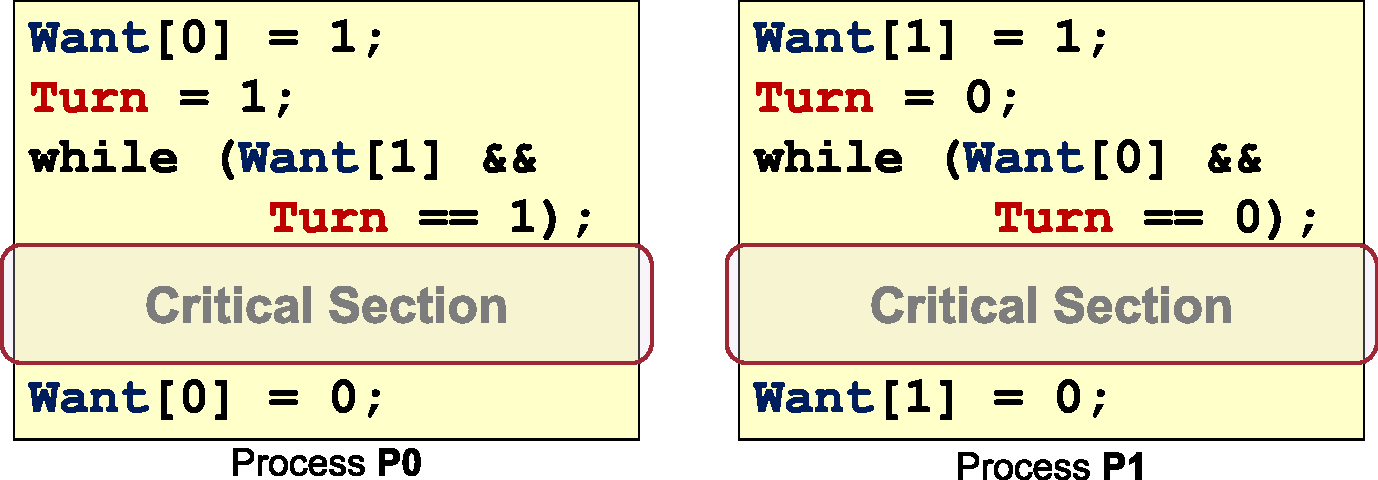
\includegraphics[width=\columnwidth]{petersons.pdf}

Disadvantages: busy-waiting, low-level, and not general

\sldef{Semaphore}: high-level mechanism; provides a way to block some processes, and unblock some sleeping processes. A semaphore contains an integer value, and can be initialised with any non-negative values.

Two atomic operations: \begin{slinenum}
\item \sldef{wait}: decrement \(S\); if now \(S < 0\), blocks
\item \sldef{signal}: increments \(S\); wakes up one sleeping process if any; never blocks
\end{slinenum}.

Semaphore invariant: \(S_{\text{current}} = S_{\text{initial}} + \text{no. signal()s} - \text{no. wait()s}\)

A binary semaphore is limited to 0 or 1; a general semaphore (\(S \ge 0\) can be implemented by a binary semaphore.

\sldef{Conditional variable}: allow tasks to wait for an event to happen; another task can signal one waiting task, or broadcast to all waiting tasks. Note: different from semaphore as if no tasks are waiting, signalling has no effect. (A task that later waits will still block.)

\section{Synchronisation problems}
\sldef{Producer-consumer}: producer produces only when buffer is not full; consumer consumes only when buffer is not empty.

\sldef{Reader-writer}: readers can share, writers must have exclusive excess.

\sldef{Dining philosophers}: Tanenbaum solution: diners signal their left and right if they are waiting. Partial order solution: number chopsticks 1 to 5; always pick up lower-numbered chopstick.

pthread provides a mutex \texttt{pthread\_mutex} with \texttt{pthread\-\_\-mutex\-\_\-(un)lock()}, and a conditional variable \texttt{pthread\_cond} with \texttt{pthread\-\_\-cond\-\_\-\{wait\-,\-signal\-,\-broadcast\}()}.

\chapter{Memory}
\sldef{Memory hierarchy}: registers ~1 ns access; cache ~10 ns access; RAM ~100 ns; HDD ~10 ms.

\section{Abstractions}
\sldef{No memory abstraction}: memory access is straightforward, but there is no way to protect one process's memory from other processes, and if two processes access the same addresses, they will conflict.

\sldef{Relocation}: offset all references in a process. \problems: slow loading time; need to somehow identify memory addresses from other normal integers.

\sldef{Base and limit}: compile all memory references to be an offset from the base register. Check all accesses against the limit register. \problems: every access involves an addition and comparison.

\sldef{Logical address}: translated to physical address by hardware or OS.

\section{Contiguous memory management}
\sldef{Fixed partitioning}: divide physical memory into a fixed number of equal partitions. \benefits: easy to manage; fast allocation. \problems: partition size must be big enough to fit the largest process; smaller processes waste memory i.e. internal fragmentation.

\sldef{Dynamic partitioning}: partitions created based on the needs of each process. \benefits: flexible; removes internal fragmentation. \problems: need to maintain more information; need to locate appropriate region when allocation; tends to lead to a large number of holes with many processes created and terminated i.e. external fragmentation.

\sldef{Dynamic partitioning algorithm}: find a hole, then split the hole. To find a hole: \begin{slinenumor}
\item first-fit: find the first hole large enough
\item best-fit: find the smallest hole large enough
\item worst-fit: find the largest hole
\item buddy system
\end{slinenumor}.

\sldef{Buddy system}

\includegraphics[width=\columnwidth]{buddysystem.pdf}

\sldef{Storage}: an array of linked lists \texttt{A[0..=K]} where \(2^K\) is the largest block size, and \texttt{A[N]} tracks the address of free blocks of size \(2^N\). \sldef{Allocating} \(N\) bytes: find the smallest \(S\) s.t. \(2^S \ge N\). Access \texttt{A[S]}; if a free block exists, use that, else find the smallest \(R \in [S+1, K]\) s.t. \texttt{A[R]} has a free block, then split that block repeatedly to get a new free \(2^S\)-byte block. \sldef{Deallocating} a block B: check \texttt{A[S]} for B's buddy; if buddy is free, merge and repeatedly merge where buddies exist. Otherwise insert B to \texttt{A[S]}.

Two blocks are size \(2^S\) buddies if their address's \(S\)th (0-based) bits are complements and the leading bits up to that bit are the same.

\section{Disjoint memory management}
\subsection{Paging}
Divide physical memory into \sldef{physical frames} of fixed size; logical memory split into \sldef{logical pages} of equal size; at runtime, pages are loaded into any available logical frames.  \sldef{Implementation}: \sldef{page table} to map logical addresses to physical. Optimise this by keeping page size a power of 2; then the page/frame number is just the most significant bits of the address.

\benefits: logical memory remains contiguous, but occupied physical memory can be discontinuous. No more external fragmentation: all free frames can be used. \problems: Internal fragmentation: logical memory space may not be a multiple of page size.

Paging can be done in pure software, with a page table stored with the process information. \problems: two accesses required for every memory reference: one to get the frame number, one for the actual memory access.

Modern processors provide a \sldef{translation lookaside buffer} which optimises this. On context switch, the TLB is flushed. The average memory access time with TLB is \(P (T_t + T_m) + (1 - P) (T_t + 2T_m)\) where \(P\) is the TLB-hit rate, \(T_t\) is the TLB access time, and \(T_m\) is the memory access time, ignoring the TLB insertion time and CPU caching.

Paging can be extended to provide memory protection with access rights (R/W/X) (e.g. for shared R/X code frames) and page validity (to check for out-of-bounds access), attached to each page table entry.

\subsection{Segmentation}
Separate memory into separate segments with a name and a limit. All memory references must be specified as a segment and offset.

Each segment is mapped to a contiguous physical memory region with a base address and a limit, and the logical address is the pair of segment and offset.

\benefits: Each segment is independent and contiguous, so they can be resized and protected independently. \problems: Needs variable-size contiguous memory regions, so it can lead to external fragmentation.

\sldef{Segmentation with paging}: each segment is now composed of pages instead of one contiguous region. A segment can grow by allocating a new page to the segment.

\section{Virtual memory}
...allows processes' logical memory to exceed the size of physical memory. This can be done by extending paging: now, some pages can be "paged out" to secondary storage.

When a page is accessed, the OS needs to check if the page is in memory, and if not (\sldef{page fault}), load the page into memory.

Virtual memory exploits the locality principle. Temporal: after a page is loaded, it is likely to be accessed again. Spatial: a page contains contiguous locations likely to be accessed again.

\section{Page table structures}
Note: each process must have its own page table!

\sldef{Direct paging}: just have all entries in a single table, for each process. \problems: waste of space since most processes do not use the full range of virtual memory.

\sldef{2/multi-level paging}: split the page table into regions; regions are allocated as needed. Need a "region table" to track regions; regions can also be identified by bit-prefixes, like pages. \benefits: less overhead. \problems: more indirection.

\sldef{Inverted page table}: map frame number to process and page number. \benefits: only one table for all processes. \problems: very slow translation.

\section{Page replacement algorithms}
If there is no free frame during a page fault, a page needs to be evicted.

\sldef{Local and global replacement}: if only a page owned by the page fault-causing process can be evicted, it is \sldef{local replacement}. \benefits: frames allocated to a process are constant, but any thrashing is contained to one process; \problems: need to decide how many frames to allocate; bad decision will cause the process to thrash.

If any page can be evicted, it is \sldef{global replacement}. \benefits: processes that need more frames can get it from other processes; \problems: badly-behaving processes hinder others, possibly causing other processes to thrash.

A good algorithm will minimise the number of page faults. The best algorithm replaces the page that will not be used again for the longest time; but this is impossible because future knowledge of memory references is needed. We use this as a basis of comparison.

\sldef{FIFO}: evict the oldest page; can be implemented using a queue. \problems: Belady's anomaly: more pages leads to more page faults, because FIFO does not exploit temporal locality.

\sldef{Least recently used} (LRU): makes use of temporal locality; replace the page that has not been used for the longest. \benefits: good results generally. \problems: hard to implement; need to keep track of last use. Can use a counter, but then to evict all pages need to be checked to find the oldest, and the counter can overflow. Can use a stack, but it is not a pure stack: entries can be removed from anywhere in the stack.

\sldef{Second-chance} (CLOCK): modified FIFO: have a "referenced bit" in each PTE, and a "next victim" pointer in a circular queue. When a page is referenced, set the bit; when a page is to be evicted, if the next victim's bit is set, unset and advance, and repeat; else evict that page.

\sldef{Working set model}: a model to determine the number of frames to allocate to a process. \(W(t, D)\) denotes the set of pages referenced in the past \(D\) time units from \(t\). By allocating just enough frames for the pages in \(W\), we reduce page faults.

\end{document}
